\chapter{Introdução} \label{Introducao}

\section{Endereços e Geocodificação}
 
\epigraph{Quase tudo o que acontece, acontece em algum lugar. Saber o local onde algo acontece pode ser fundamental.}{\cite{longley2013}}

No livro de \cite{longley2013}, os autores exploram a relação entre a humanidade e a localização. Para eles, é evidente que a maior parte das atividades humanas ocorre no planeta Terra, e, portanto, a vida está profundamente ligada à localização. Assim sendo, compreender e manipular informações geográficas é essencial para qualquer aplicação que envolva a humanidade. Além disso, os autores explicam que decisões importantes podem ter consequências geográficas. Um exemplo disso seria uma transação financeira que, em casos extremos, poderia desencadear uma crise econômica em uma região específica.

No artigo de \cite{Zamberg2009}, o autor apresenta aspectos relevantes das informações geográficas que complementam o que foi mencionado anteriormente. Segundo ele, o endereço é a principal maneira de conceitualizar a localização no mundo atual. Isso ocorre devido ao fato de os endereços serem utilizados em diversas aplicações de diferentes áreas de estudo, como na saúde \cite{AmericaJournal2001, Kypri2009, Mazumdar2008}, nas ciências sociais \cite{Chow2011}, na análise criminal ou judiciária \cite{Olligschlaeger1998}, na análise ambiental \cite{Gilboa2006}, na ciência da computação \cite{Zamberg2009}, na economia \cite{Whitsel2006} e em outros campos.

Para atingir esse objetivo, é necessário criar uma representação computacional do endereço para que as aplicações possam utilizá-la. A representação mais comum, conforme \cite{Zamberg2009}, é a utilização de coordenadas x e y em um plano, geralmente representando latitude e longitude. Esse processo de transformação em um endereço nessas coordenadas é chamado de Geocodificação ou Georreferenciamento. De acordo com \cite{Zamberg2009}, esse processo envolve três etapas:

\begin{itemize}
   \item Processamento do endereço de entrada: o endereço é lido, dividido em componentes (rua, número, bairro, etc.), padronizado e cada campo é atribuído a uma categoria; por fim, as categorias necessárias são indexadas.
   \item Busca na base de referência: com base no algoritmo escolhido, é realizada uma busca na base de referência para selecionar e classificar potenciais candidatos como resposta.
   \item Seleção do(s) candidato(s) para resposta: após a busca, a classificação gerada é analisada e os melhores candidatos são selecionados.
\end{itemize}

De acordo com \cite{longley2013}, além de representar um endereço computacionalmente, o georreferenciamento utilizando latitude e longitude oferece várias vantagens:

\begin{itemize}
   \item Precisão espacial: é capaz de indicar com alta precisão a localização de um determinado endereço.
   \item Cálculos de distância: como é um sistema espacial, permite a obtenção de distâncias e, por consequência, o cálculo de outras métricas para o endereço.
   \item Compreensão global: é um sistema usado mundialmente e, geralmente, é mais fácil de identificar e entender.
\end{itemize}

Apesar de todas as vantagens e aplicações, o processo de geocodificação pode levar a informações incorretas. No livro de \cite{longley2013}, os autores chamam essas discrepâncias de "incertezas". Para compreender o que é a incerteza, é necessário considerar outros aspectos das falhas de informação. Nesse contexto, são introduzidos os seguintes conceitos:

\begin{itemize}
   \item Erro: a diferença entre o observado e o obtido.
   \item Falta de acurácia: a diferença entre a realidade e nossa representação dela.
   \item Ambiguidade: quando um único valor está presente em mais de um objeto.
   \item Indefinição: a falta de informações necessárias.
\end{itemize}

Após definir esses termos, os autores definem a incerteza como: "a medida da compreensão do usuário sobre a diferença entre o conteúdo de um conjunto de dados e os fenômenos reais que os dados devem representar" \cite{longley2013}. Em outras palavras, a incerteza é uma medida que descreve o nível de compreensão do usuário em relação ao conjunto de dados obtidos e à realidade que esses dados têm a intenção de representar. A figura \ref{fig:incerteza} apresenta uma visão conceitual da incerteza, onde cada processo muda um pouco a realidade, sendo assim a representação final tem sempre um nível de incerteza. A partir dessa perspectiva, a incerteza foi aceita como uma métrica apropriada para avaliar a qualidade dos Sistemas de Informação Geográfica (SIG).

\begin{figure}[ht]
   \centering
   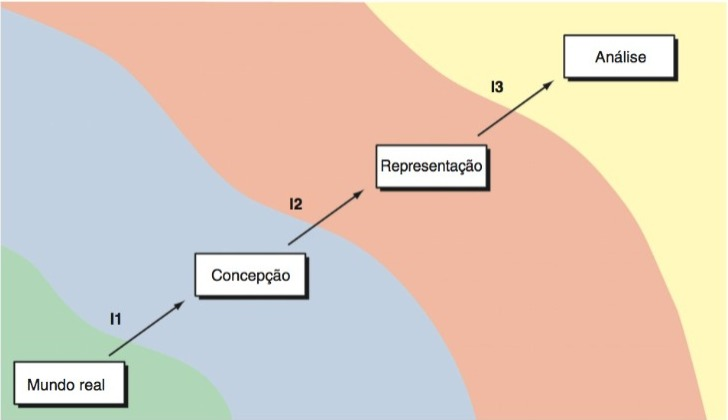
\includegraphics[width=0.8\textwidth]{Figuras/incertezaLivro.jpeg}
   \caption{Retirada do livro \cite{longley2013}. Visão conceitual da incerteza, onde os filtros I1, I2, I3 distorcem a informação original}
   \label{fig:incerteza}
\end{figure}

\section{APIs de Geocodificação e Análise de qualidade}

Atualmente, no TerraLAB - Laboratório de Pesquisa e Capacitação em Software \cite{terralab}, utilizamos informações geográficas para o desenvolvimento de nossas aplicações. Esses aplicativos utilizam endereços geocodificados para criar mapas, rotas, áreas de abrangência, relatar locais, divulgar eventos, entre outras funcionalidades. Isso ressalta a grande importância da geocodificação e como a qualidade desse processo impacta significativamente o que é produzido em nosso laboratório.

Para adquirir informações relacionadas a endereços, fazemos uso da geocodificação obtida por meio de APIs online de geocodificação.

Por muitos anos, a principal maneira de obter informações geográficas era através de software SIG. Conforme \cite{stein2021geoprocessamento}, um Sistema de Informação Geográfica (SIG) é um conjunto de ferramentas capazes de analisar e integrar dados geográficos, permitindo acesso fácil a dados para os usuários, sem depender de ferramentas como o GPS.

Segundo \cite{Chow2016}, embora os SIG tenham sido a ferramenta convencional por muitos anos, utilizar esse método para geocodificação requer um profissional capacitado. A ferramenta demanda o pré-processamento dos dados, criação de um localizador de endereços, customização de parâmetros, controle de qualidade e correção manual de falhas. Todo esse processo é custoso para o usuário comum. Por essa razão, a geocodificação utilizando ferramentas online retira do usuário grande parte da responsabilidade, como a manutenção da base, tornando assim o processo de obtenção de informações menos oneroso.

Apesar de a geocodificação online ser mais simples de utilizar, para que o SIG seja substituído por ela, deve-se considerar sua qualidade em relação à qualidade do SIG. No artigo \cite{Chow2016}, são avaliadas oito ferramentas de geocodificação, sendo duas delas SIGs e as demais ferramentas da internet. As ferramentas utilizadas foram: SRI ArcGIS Address Locator, CoreLogic PxPoint, Google Maps API, Yahoo! PlaceFinder, Microsoft Bing, Geocoder.us, Texas A and M University Geocoder e OpenStreetMap (OSM). Para calcular o erro, uma base de referência foi utilizada, contendo informações descritivas do endereço (rua, número, cidade etc.) e informações geográficas (latitude e longitude). Essa base é considerada a referência, pois os dados de latitude e longitude foram obtidos manualmente (por GPS ou pesquisa manual). Chamaremos essa e outras bases de referência de "base padrão ouro". A base em questão contém 940 endereços do estado do Texas, Estados Unidos da América (EUA), sendo que 78 destes são da região Central Texas, região considerada importante para o autor. O erro de cada endereço geocodificado foi calculado da seguinte forma:

\begin{align}
   \epsilon_x &= x_{\text{ref}} - x_{\text{geoc}} \\
   \epsilon_y &= y_{\text{ref}} - y_{\text{geoc}} \\
   \varepsilon_{xy} &= \sqrt{\epsilon_x^2 + \epsilon_y^2}
\end{align}

Onde:
\begin{itemize}
   \item $\epsilon_x$ é o erro da longitude,
   \item $\epsilon_y$ é o erro da latitude,
   \item $\varepsilon_{xy}$ é o erro euclidiano.
\end{itemize}
   
O estudo evidenciou que não há diferença significativa entre as ferramentas online e os SIGs. Tanto os SIGs quanto as ferramentas online apresentaram média e desvio padrão de erro semelhantes. Além disso, a taxa de resposta (ou seja, quantos endereços receberam uma resposta da ferramenta utilizada) variou entre 97,8\% e 100\%, o que é considerado satisfatório. Dessa forma, o estudo obteve êxito ao demonstrar que as ferramentas online podem ser utilizadas como substitutas dos SIGs.

Apesar de \cite{Chow2016} ter apresentado resultados significativos, o estudo apresenta algumas limitações. A principal delas é a quantidade de dados utilizada para a avaliação, além do foco restrito a uma única região (Texas, EUA). O presente trabalho busca abordar essas limitações ao conduzir a análise em uma região diferente do mundo, com ênfase no Brasil, e ampliar a quantidade de dados avaliados. Entretanto, nosso enfoque será exclusivamente em ferramentas de geocodificação online (GeoAPIs), considerando que elas já estão consolidadas no mercado e na academia.

Outro estudo importante é \cite{Clodoveu2011}, que faz uma avaliação da qualidade da geocodificação do Google Maps API fornecida pelo Google Cloud Platform \cite{GCP}. Nesse estudo, os autores utilizam uma base padrão ouro com os dados de Belo Horizonte, cidade de Minas Gerais, estado do Brasil para essa avaliação. A base conta com mais de 540 mil endereços da cidade e é mantida pela empresa de informática e informação do município de Belo Horizonte - Prodabel \cite{Prodabel}. A empresa atualiza os dados mensalmente e tem parceria com outras 26 empresas para manter a base o mais correta possível. Ela conta com informações descritivas, sociais e espaciais do endereço. Para medir o erro, foi calculada a distância euclidiana dos pontos geocodificados para os pontos originais. A partir do erro, o estudo faz análises espacias do erro e também relaciona a acurácia descrita pela API com o erro gerado. O estudo mostrou que o Google Maps API tem taxa de acerto de 74,7\%, considerando que acertou se o erro for menor de 150 metros. Outra descoberta foi que o erro é menor nas áreas centrais da cidade, e maior na periferias. Os autores também tentaram fazer uma relação entre erro e renda, porém não foi possível vizualizar nenhuma relação direta.

Apesar das descobertas importantes, o estudo apresenta limitações notáveis. Primeiramente, ele se restringe à análise de apenas uma API de geocodificação. Além disso, o estudo se concentra exclusivamente em uma cidade brasileira, o que restringe a generalização dos resultados. Para abordar essas limitações, nosso trabalho atual visa expandir a análise. Planejamos examinar uma amostra da mesma base de dados, utilizando diferentes APIs de geocodificação. Além disso, nossa pesquisa incluirá uma análise de uma base de dados da região metropolitana de São Paulo, proporcionando uma maior diversidade ao nosso estudo.

\section{Objetivos}

O principal objetivo deste trabalho é avaliar o erro, a discrepância e a acurácia de cinco APIs utilizadas no laboratório de pesquisa e capacitação em desenvolvimento de software - TerraLAB. As APIs em análise são: Google Maps, TomTom, Open Route Service (ORS), Mapbox e Here. O erro será analisado em relação às respostas fornecidas pelas APIs, verificando o quanto diferem das esperadas. A discrepância medirá o nível de discordância entre as APIs. Por fim, a acurácia será utilizada para verificar a precisão das respostas fornecidas por essas APIs.
    
Uma parte essencial deste trabalho é compreender os pontos em que essas APIs apresentam falhas. Portanto, a análise espacial dessas medidas terá grande destaque na pesquisa.

Com isso, gostaríamos de responder as seguintes perguntas:
\begin{itemize}
   \item Qual API das utilizadas apresenta mais erros?
   \item Existe algum padrão espacial nos erros?
   \item Alguma medida de variância entre as APIs (discrepância) está relacionada aos erros?
\end{itemize}

Para alcançar essas respostas, temos objetivos específicos a serem cumpridos:

\begin{itemize}
   \item Coletar bases de dados padrão-ouro.
   \item Calcular as medidas para avaliação.
   \item Avaliar a distribuição das medidas.
   \item Correlacionar as medidas.
   \item Avaliar de que forma o espaço se relaciona com essas medidas.
\end{itemize}






